\documentclass{standalone}
% \usepackage{tikz}
\usepackage{LILLYxCOLOR}
\usepackage{LILLYxGRAPHICS}
\usepackage{enumitem}     

\usetikzlibrary{3d}

\begin{document}
    %#1: x, #2: y, #3: color, #4: name for top center
    \def\Reader#1#2#3#4{
        \draw[fill=#3,fill opacity=0.8] (#1-0.2,0,0.2+#2) -- ++(0,0.5,0) -- ++(0,0,-1.4) -- ++(0,-0.5,0) -- cycle;
        \draw[fill=#3,fill opacity=0.8] (#1-0.2,0,0.2+#2-1.4) -- ++(0,0.5,0) -- ++(1.4,0,0) -- ++(0,-0.5,0) -- cycle;
        \fill[#3,opacity=0.1] (#1-0.2,0,0.2+#2) -- ++(0,0.5,0) -- ++(1.4,0,0) -- ++(0,-0.5,0) -- cycle;
        \fill[#3,opacity=0.1] (#1-0.2+1.4,0,0.2+#2) -- ++(0,0.5,0) -- ++(0,0,-1.4) -- ++(0,-0.5,0) -- cycle;
        \draw (#1-0.2+1.4,0,0.2+#2) -- ++(0,0.5,0);
        
        \draw[canvas is xz plane at y=0] (#1-0.2,0.2+#2) rectangle ++(1.4,-1.4);
        \draw[canvas is xz plane at y=0.5,fill=#3,fill opacity=0.1] (#1-0.2,0.2+#2) rectangle ++(1.4,-1.4) node[midway,centered] (#4) {};
    }
    \def\MainControllerUnit#1#2#3#4{
        \draw[black,fill=MudWhite] (#1) -- ++(-#2,0,0) -- ++(0,-#3,0) -- ++(#2,0,0) -- cycle;
        \draw[black,fill=MudWhite] (#1) -- ++(0,0,-#4) -- ++(0,-#3,0) -- ++(0,0,#4) -- cycle;
        \draw[black,fill=MudWhite] (#1) -- ++(-#2,0,0) -- ++(0,0,-#4) -- ++(#2,0,0) -- cycle; 
        \coordinate (mcu) at ($(#1)+(-#2/2,0,-#4/2)$);
        \coordinate (mcu-front) at ($(#1)+(-#2/2,-#3/2,0)$);
        \node[yslant=1.1] at ($(#1)+(0,-#3/2,-#4/2)$) {FPU};
    }
    \def\Connector#1#2#3#4{
        \fill[#1!96!black] (#2)++(-0.15,-0.15) rectangle ++(0.3,0.3);
        \draw[#1,very thick] (#2) #3 -- (#4);
        \fill[#1] (#4) circle [radius=3.5pt];
    }
    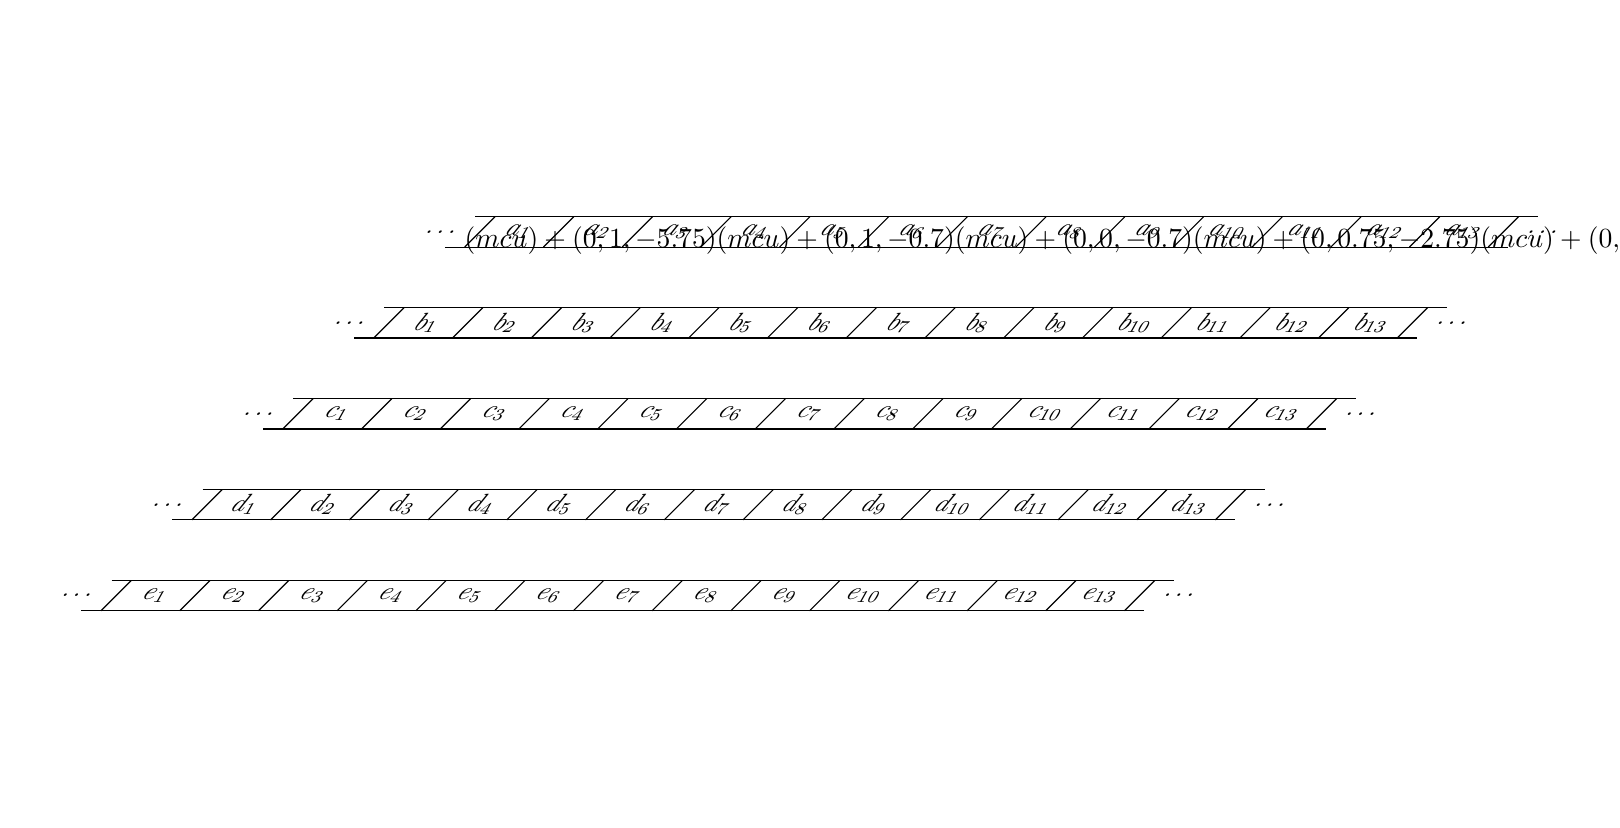
\begin{tikzpicture}[line join=round]
        \begin{scope}[canvas is xz plane at y=0]
            \foreach \y/\lbl in {0/a,3/b,6/c,9/d,12/e} {
                \draw (-0.25,\y) -- (13.25,\y);
                \draw (-0.25,\y-1) -- (13.25,\y-1);
                % verts
                \foreach[count=\i] \a in {\ldots,\lbl_1,\lbl_2,\lbl_3,\lbl_4,\lbl_5,\lbl_6,\lbl_7,\lbl_8,\lbl_9,\lbl_{10},\lbl_{11},\lbl_{12},\lbl_{13},\ldots} {
                    \ifnum\i>1 \draw (\i-2,\y) -- ++(0,-1); \fi
                    \node[xslant=0.56] at(\i-1.5,\y-0.5) {\small\(\a\)};
                }
            }    
        \end{scope}
        % readers
        \Reader{9}{0}{AppleGreen}{a}
        \Reader{6}{3}{Crimson}{b}
        \Reader{3}{6}{Azure}{c}
        \Reader{11}{9}{Purple}{d}
        \Reader{6}{12}{ChromeYellow}{e}

        % controller unit
        \MainControllerUnit{16,0,6}{2}{1}{4}

        % connect em a/apple green first
        \Connector{AppleGreen}{a}{-- ++(0,1,0) -- ($(mcu)+(0,1,-5.75)$) -- ($(mcu)+(0,1,-0.7)$)}{$(mcu)+(0,0,-0.7)$}
        \Connector{Crimson}{b}{-- ++(0,0.75,0) -- ($(mcu)+(0,0.75,-2.75)$) -- ($(mcu)+(0,0.75,-1.5)$)}{$(mcu)+(0,0,-1.5)$}
        \Connector{Azure}{c}{-- ++(0,0.75,0) -- ($(mcu)+(0,0.75,0.2)$)}{$(mcu)+(0,0,0.2)$}
        \Connector{Purple}{d}{-- ++(0,0.75,0) -- ++(0,0,-2.09) -- ($(mcu)+(0,0.75,1.1)$)}{$(mcu)+(0,0,1.1)$}
        \Connector{ChromeYellow}{e}{-- ++(0,1,0) -- ($(mcu-front)+(0,1,3)$) -- ++(0,-1,0)}{mcu-front}
        % \Connector{Crimson}{b}{-- ++(0,1,0) -- ($(mcu)+(0,1,0)$)}{mcu}
        % \Connector{Azure}{c}{-- ++(0,1,0) -- ($(mcu)+(0,1,0)$)}{mcu}
        % \Connector{Purple}{d}{-- ++(0,1,0) -- ($(mcu)+(0,1,0)$)}{mcu}
        % \Connector{ChromeYellow}{e}{-- ++(0,1,0) -- ($(mcu)+(0,1,0)$)}{mcu}
        % border nodes:
        \node[above=2.15cm] at(current bounding box.north) {};
        \node[below=2.15cm] at(current bounding box.south) {};
        \node[right] at(current bounding box.east) {};
        \node[left] at(current bounding box.west) {};
    \end{tikzpicture}
\end{document}
